\chapter{LED Controller}

\section{Task Description}

To drive the sixteen board LEDs with \texttt{ledcntrl\_top.sv} using appropriate registers (\texttt{INT\_CLR}, \texttt{INT\_MASK},
\texttt{INT\_STAT}, \texttt{INT\_MASKED}, \texttt{CTL} and \texttt{CFG}) and
provide linting and synthesis results.

\section{Figures}

\begin{figure}[H]
  \centering
  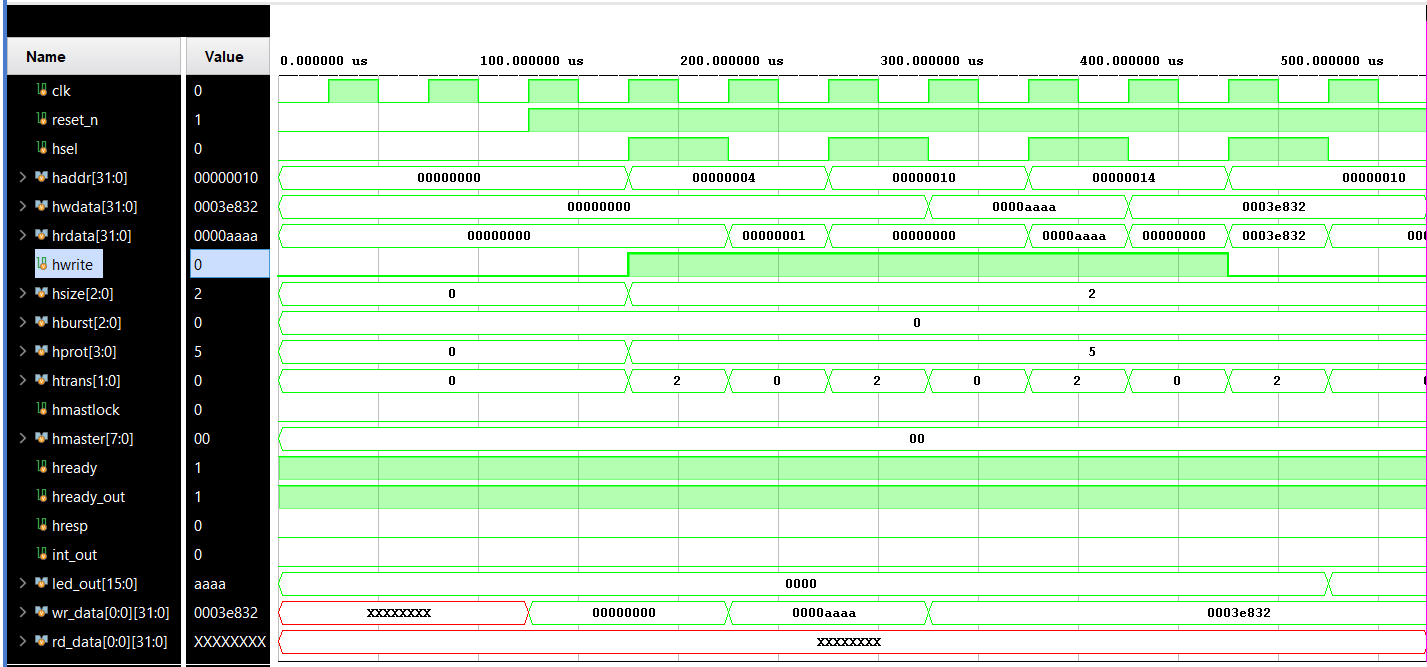
\includegraphics[width=\linewidth]{figures/Lab3/led_setup.png}
  \caption{AHB writes to INT\_MASK, CTL and CFG, followed by readback of CTL and CFG.}
  \label{fig:led-setup}
\end{figure}

\evidencefigure{led-waveform.png}{LED controller PWM and interrupt sequence.}{fig:led-waveform}{Capture the LED simulation showing the alternate LED mask, PWM period and duty cycle, and interrupt assertion and clear.}

\begin{figure}[H]
  \centering
  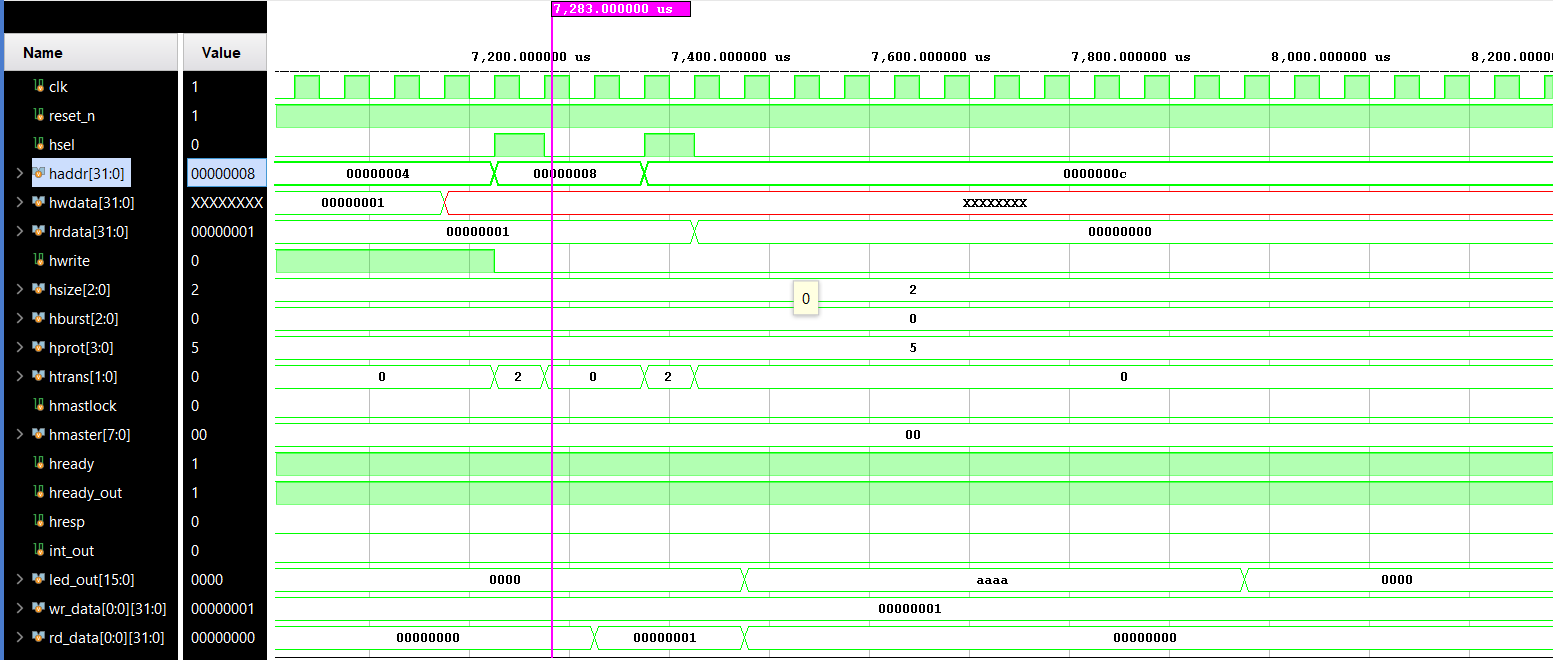
\includegraphics[width=\linewidth]{figures/Lab3/led_mask_test.png}
  \caption{Interrupt masked: INT\_STAT reads 1 and INT\_MASKED reads 0, while \texttt{int\_out} stays low as PWM periods keep ending.}
  \label{fig:led-mask}
\end{figure}

\begin{figure}[H]
  \centering
  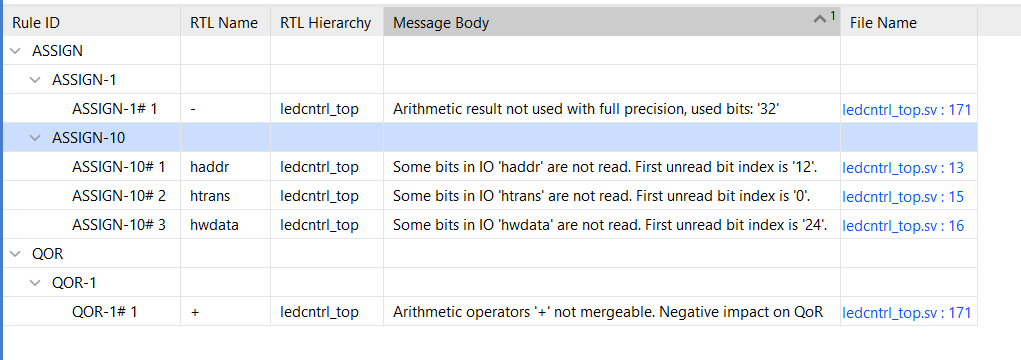
\includegraphics[width=\linewidth]{figures/Lab3/Lab03_ledcntrl_linter.png}
  \caption{Vivado lint findings for the LED controller.}
  \label{fig:led-lint}
\end{figure}

\section{Discussion}

\texttt{led\_tb.sv} uses the AHB-Lite master to unmask the interrupt,
set \texttt{CTL} to \texttt{0xAAAA}, and set \texttt{CFG} to
\texttt{0x0003E832} for 1\,kHz PWM at 50\% duty cycle. It reads the control
and configuration registers, waits for the interrupt, writes one to
\texttt{INT\_CLR}, and waits for the interrupt to go low.

The Vivado linter reported five findings for \texttt{ledcntrl\_top}, shown in
Fig.~\ref{fig:led-lint}. All of them are intended by the design.

Three \texttt{ASSIGN-10} findings flag input bits that are never read. Only
\texttt{haddr[11:0]} is decoded, because the register offsets fit in the
lowest 12 address bits and the upper bits select the slave in the
interconnect. Only \texttt{htrans[1]} is checked, because this bit alone
separates a valid transfer (\texttt{NONSEQ} or \texttt{SEQ}) from an idle
cycle. Only \texttt{hwdata[23:0]} is used, because the widest register,
\texttt{CFG}, holds the frequency in bits~23--8 and the duty cycle in
bits~7--0.

The \texttt{ASSIGN-1} and \texttt{QOR-1} findings both refer to line~171,
where the phase accumulator subtracts \texttt{CLK\_FREQ\_HZ} at the end of a
PWM period. The sum is computed with 33~bits to hold the carry, and the
result is stored in the 32-bit accumulator. No information is lost, because
the result is always smaller than \texttt{CLK\_FREQ\_HZ}. The
\texttt{QOR-1} note only states that this subtraction and the preceding
addition are built as two separate adders.
